\section{Auswertung}
\label{sec:Auswertung}

\section{Verwendete Stäbe}
\label{sec:Stäbe}

Es werden ein Stab mit rundem und ein Stab mit quadratischem Querschnitt verwendet. Der runde Stab besitzt einen Durchmesser $d$ von $10mm$ bei einer Länge $l_{r}$ von $57.5cm$ und einer Masse $m_{r}$ von $379.2g$.
Für den eckigen Stab wurden die nötigen Daten wie folgt ermittelt:

\begin{equation*}
  a = 10mm \\
  l_{q} = 60cm \\
  m_{q} = 502.4g \\
\end{equation*}

Hierbei bezeichnet $a$ die Kantenlänge des Querschnittes. Hieraus ergeben sich die Dichten $\rho_{r} = 8396.7\frac{kg}{m^3}$ und $\rho_{q} = 8373.3\frac{kg}{m^3}$. Dies entspricht etwa der Dichte von  Messing CuZn39Pb3 von $\rho_{Messing} = 8.47\frac{g}{cm^3}$ \cite{DKI}. Es wird dementsprechend davon ausgegangen, dass es sich bei beiden Stäben um Messingstäbe handelt, welche ein Elastizitätsmodul von ca. $E_Messing = 97 \frac{kN}{mm^3}$ \cite{DKI} aufweisen sollten.

\subsection{Einseitige Einspannung}
\label{sec:Einseitig}

\begin{table}
  \centering
\caption{Auslenkung des runden Stabes}
\label{tab:rund}
\sisetup{round-mode = places , round-precision = 2}
\begin{tabular}{S S S S}
  \toprule
  {$x/cm$} & {$y/mm$} & {$y'/mm$} {$\delta y/mm$}\\
  \midrule
  include('../Werte/V103-Reihe1-tab.txt')
\bottomrule
\end{tabular}
\end{table}
\FloatBarrier

Die bei einseitiger Einspannung des runden Stabes ermittelten Werte lassen sich der Tabelle \ref{tab:rund} entnehmen, wobei $y$ die Auslenkungen im unbelasteten Fall darstellt, $y'$ die im belasteten und $x$ die Position entlang des Stabes (Einspannung bei $x=0$). Hierbei wurde eine Belastung von $m_1 = 379.2g$ gewählt.

\begin{figure}
  \centering
  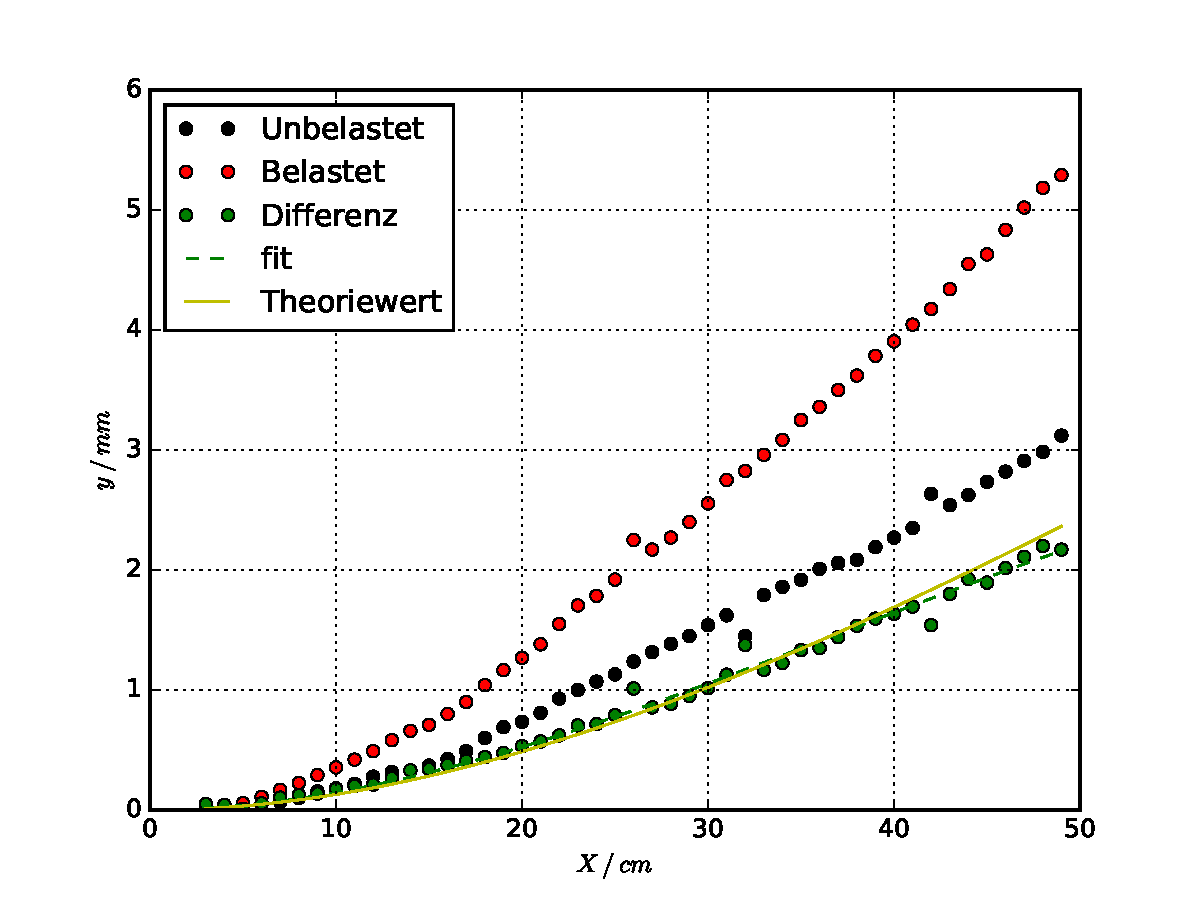
\includegraphics{/Plots/Reihe1.pdf}
  \caption{Reihe1}
  \label{fig:Reihe1}
\end{figure}

\begin{figure}
  \centering
  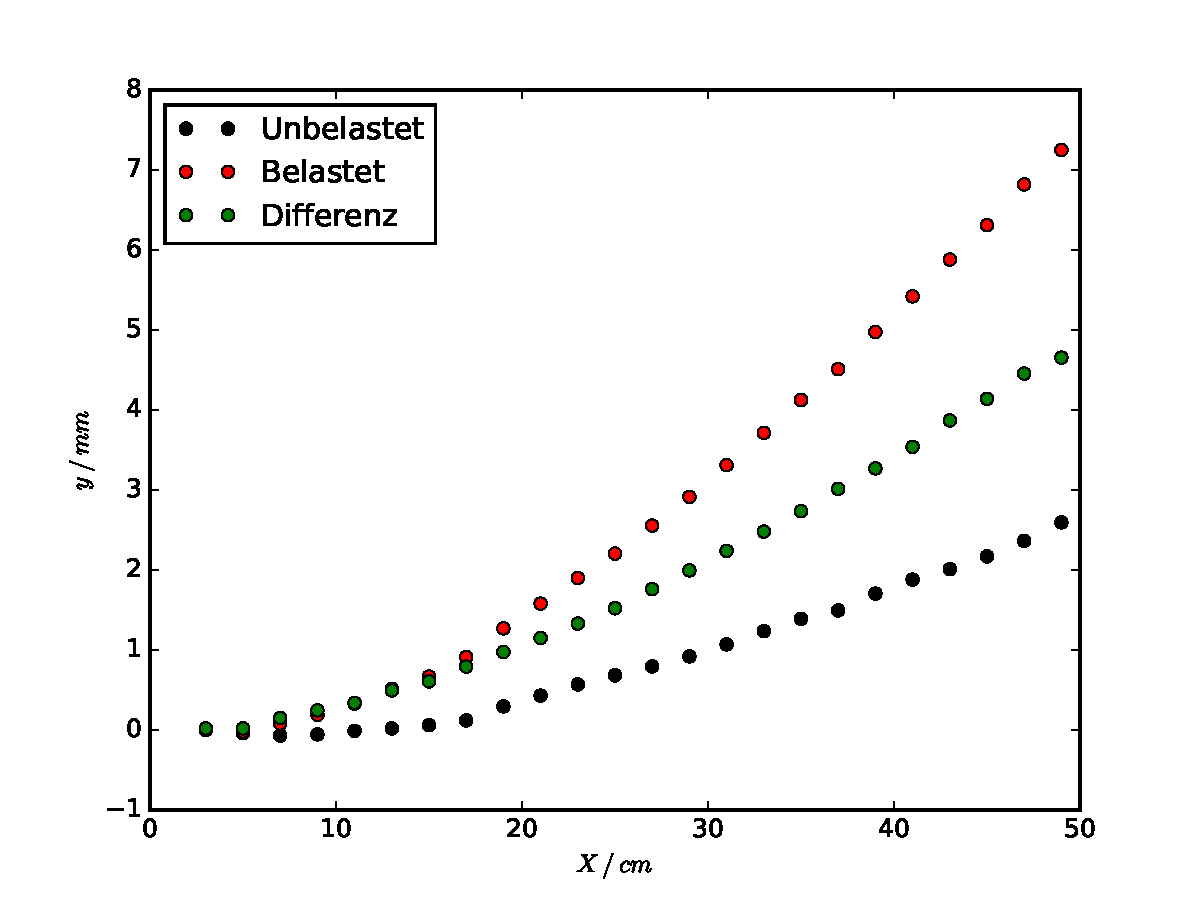
\includegraphics{/Plots/Reihe2.pdf}
  \caption{Reihe2}
  \label{fig:Reihe2}
\end{figure}

\begin{figure}
  \centering
  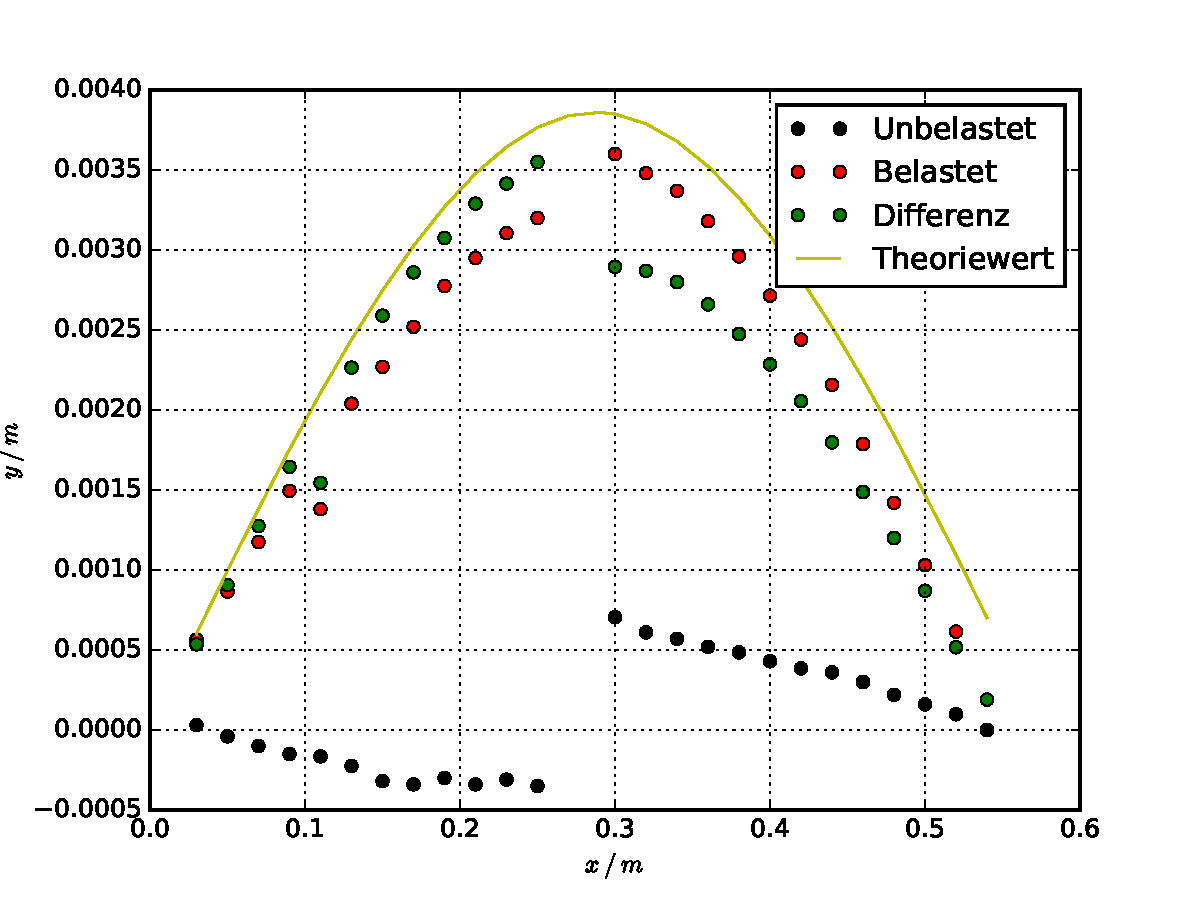
\includegraphics{/Plots/Reihe3.pdf}
  \caption{Reihe3}
  \label{fig:Reihe3}
\end{figure}
